\documentclass[11pt]{article}
\usepackage[margin=0.8in]{geometry}
\usepackage{lmodern}
\usepackage{graphicx}
\usepackage{booktabs}
\usepackage[hyphens]{url}
\usepackage{amsmath}
\usepackage{hyperref}
\usepackage{caption}

\title{Group Assignment: Project Update\\
\large Scene-Disjoint Real-CE Adaptation and Text-Region Cross-Noise Consistency LoRA for DoSSR}
\author{Team 1 (LEMMEPASS)\\
Hoang Nguyen Anh (25125002), Huynh Tran Gia Han (25125042),\\
Ho Quang Minh (25125060), Nguyen Phan Minh Nhat (25125033)\\
SC203 Scientific Methods, Class 25A02}
\date{November 2026}

\begin{document}
\maketitle

\begin{abstract}
Building on our earlier baseline experiments on \texttt{RealSRVal\_crop128}, this report covers our Phase-2 work on the real-world $4\times$ \texttt{Real-CE} benchmark ($945$ total pairs = $645$ official train + $300$ untouched val). Using a scene-disjoint $80/20$ split of the train set, we evaluate on 30 validation patches (154 text boxes; 63 HR-solvable) with \texttt{--rec-only} RapidOCR across 10 inference seeds. We inject rank-8 LoRA adapters into DoSSR and train with a text-masked cross-noise consistency loss ($\mathcal{L}_{\text{cons}}$) via a two-pass backward that adds zero extra peak VRAM ($+0.00$~GiB). Tuning $\lambda_{\text{cons}} = 0.2$ and gating consistency to $t \le 499$, \texttt{LoRA~3} beats \texttt{LoRA~2} at every checkpoint across 2,000 steps and is best at step~1,600 ($74.13\%$ Box Error on the HR-solvable boxes vs.\ $77.46\%$ for \texttt{LoRA~2}; $0.5488$ CER). However, unmodified \texttt{Base DoSSR} ($69.21\%$) still beats all LoRA runs on OCR, deterministic \texttt{Bicubic} $\times 4$ ($55.56\%$) beats all diffusion models on OCR, and $\mathcal{L}_{\text{rec}}$ stayed active on dead timesteps ($t \ge 500$).
\end{abstract}

\section{Progress Overview: What Is New Since the Earlier Baseline}
Compared to our earlier frozen-DoSSR baseline on 100 \texttt{RealSRVal\_crop128} images (25 text-positive, 193 boxes, 136 HR-solvable, \texttt{--rec-only} RapidOCR \texttt{upscale=1}), this update shifts to the $4\times$ \texttt{Real-CE} benchmark ($945$ pairs: 645 scene-split train + 300 untouched val) with 30 validation patches (154 boxes, 63 HR-solvable) scored under \texttt{--rec-only --rotate-vertical --upscale 2}. We inject rank-8 LoRA ($1{,}659{,}904$ trainable parameters across 256 tensors) and train with cross-noise consistency ($\mathcal{L}_{\text{cons}}$) via a $+0.00$~GiB two-pass backward. We also add schedule and FP32 gradient audits plus \texttt{Bicubic}, \texttt{Base DoSSR}, $\lambda_{\text{cons}}$, timestep gating ($t \le 499$), and 2,000-step runs, contrasting with related diffusion SR methods using non-uniform diffusion (CCSR~\cite{sun2024ccsr}), test-time noise fusion (PNFS~\cite{jiang2025pnfs}), or segmentation decoders (TADiSR~\cite{hu2025tadIsr}).

\section{Dataset Transition (\texttt{Real-CE} \texorpdfstring{$4\times$}{4x}) and Split Provenance}
\subsection{945-Pair Provenance and Scene-Disjoint Partitioning}
To supervise text-region consistency without touching our final test benchmarks, we adopted \texttt{Real-CE} ($13\text{mm} \to 52\text{mm}$ real optical $4\times$ smartphone zoom pairs from iPhone~11 Pro and iPhone~12 Pro). Repository dataset auditing (\path{results/realce_feasibility_summary.json} and \path{results/realce_val_split_and_category_audit.json}) establishes the exact provenance across all $945$ paired images:
\begin{itemize}
    \item \textbf{Official \texttt{RealCE/train/} ($645$ pairs):} The sole source used for model adaptation and internal validation. Running \path{scripts/split_realce_by_scene.py} (\path{--split train} \path{--scale x4} \path{--val-ratio 0.20} \path{--seed 42}) clusters captures by root scene identifier prior to $512\times 512$ patch extraction, enforcing $\text{Train scenes} \cap \text{Val scenes} = \emptyset$ (zero scene overlap).
    \item \textbf{Official \texttt{RealCE/val/} ($300$ pairs):} Kept $100\%$ untouched alongside \texttt{RealSRVal\_crop128} (100 pairs) as strictly held-out final test sets.
    \item \textbf{Internal Validation Benchmark ($30$ patches):} Thirty text-centered $512\times 512$ patches (\texttt{128x128} LR $\to$ \texttt{512x512} HR) drawn from $30$ distinct parent scenes, containing $154$ annotated text bounding boxes. Across 10 fixed validation seeds (42--51, \texttt{per\_image\_seed: true}, \texttt{disable\_sdpa: true}, \texttt{prompt\_mode: empty}), every checkpoint generates $300$ images ($1{,}540$ box-seed instances).
\end{itemize}

\subsection{Standardized OCR Scoring Protocol (\texttt{--rec-only})}
In the pilot, default RapidOCR (\texttt{det+rec}, \texttt{upscale=1}) missed tight crop borders, giving an image-mean ($n=30$) \emph{HR Ceiling} of $92.91\%$ Box Error and $0.7334$ CER (\path{results/lora_pilot_summary.json}). Re-scoring with \path{scripts/text_eval.py} (\texttt{--ocr-backend rapidocr --rec-only --rotate-vertical --upscale 2}) cuts image-mean HR error to $57.91\%$ ($0.2722$ CER), yielding a box-weighted All-154 HR Ceiling of $59.09\%$ Box Error ($0.2908$ CER) and a 63-box HR-solvable subset ($40.91\%$) where HR reaches $0.00\%$ Box Error ($0.0000$ CER).

\section{Proposed Method, Mathematical Audit, and FP32 Verification}
\subsection{Parameter-Efficient LoRA Architecture}
Upstream DoSSR combines Stable Diffusion~2.1 with ControlNet ($\sim 1{,}330\text{M}$ parameters total; full upstream training updates all $\sim 361\text{M}$ ControlNet weights). Furthermore, \texttt{ControlledUnetModel.forward} wraps the UNet encoder (\texttt{input\_blocks}) and \texttt{middle\_block} inside \texttt{with torch.no\_grad():}. Rather than modifying \texttt{external/DOSSR}, we freeze all base weights and inject low-rank adapters (\texttt{LoRALinear}, rank $r=8$, $\alpha=16.0$, scaling $\alpha/r = 2.0$, zero-initialized $B$ for exact baseline equivalence at step~0) onto the attention linear projections (\texttt{.to\_q}, \texttt{.to\_k}, \texttt{.to\_v}, \texttt{.to\_out.0}) within \texttt{control\_model.} and \texttt{model.diffusion\_model.output\_blocks.}. This yields exactly \textbf{$1{,}659{,}904$ trainable parameters} across \textbf{256 LoRA tensors}.

\subsection{Exact \texorpdfstring{$\hat{\epsilon}_\theta \to \hat{x}_0$}{epsilon to x0} Equations and \texttt{trunc\_12} Timestep Audit}
In DoSSR's \path{predict_x0_out_mix} (\path{external/DOSSR/ldm/models/diffusion/ddpm.py}, lines 909--917, \texttt{parameterization == "eps"}), given clean HR latent $x_0 = E(\text{HR})\cdot 0.18215$, RealESRNet-preprocessed LR latent $\hat{x}_{\text{LR}} = E_{\text{cond}}(\text{RealESRNet}(\text{LR}))\cdot 0.18215$, conditioning $c$, timestep $t \in \{0,\dots,999\}$, and Gaussian noise $\epsilon \sim \mathcal{N}(0, I)$:
\begin{align}
x_{\text{rect}}(t) &= \eta_t\,\hat{x}_{\text{LR}} + (1 - \eta_t)\,x_0, \label{eq:xrect} \\
x_t(\epsilon) &= \sqrt{\bar{\alpha}_t}\,x_{\text{rect}}(t) + \sqrt{1 - \bar{\alpha}_t}\,\epsilon, \label{eq:qsample} \\
\hat{\epsilon}_\theta &= \text{ControlledUNet}\!\left(x_t(\epsilon),\, t,\, c_{\text{crossattn}},\, \text{ControlNet}\big(x_t(\epsilon),\, \hat{x}_{\text{LR}},\, t,\, c_{\text{crossattn}}\big)\right), \label{eq:epshat} \\
\hat{x}_0(\epsilon) &= \frac{1}{\sqrt{\bar{\alpha}_t}}\,x_t(\epsilon) - \sqrt{\frac{1}{\bar{\alpha}_t} - 1}\;\hat{\epsilon}_\theta(x_t(\epsilon), t, c). \label{eq:x0hat}
\end{align}

Because Eq.~\eqref{eq:qsample} adds noise to $x_{\text{rect}}(t)$ rather than $x_0$, Eq.~\eqref{eq:x0hat} algebraically recovers $x_{\text{rect}}(t)$ when $\hat{\epsilon}_\theta = \epsilon$, not $x_0$ directly. Both upstream \path{ControlLDM.shared_step} (\path{external/DOSSR/model/cldm.py:353}) and our LoRA training loop (\path{scripts/run_lora_trial.py:555--560}) still compare this output (\texttt{pred\_x0}) directly against the clean HR latent $x_0$, so the model must absorb the LR-to-HR shift inside $\hat{\epsilon}_\theta$. This is also why $t \ge 500$ is a dead regime: when $t \ge 500$, $\eta_t \equiv 1.0$, so $x_{\text{rect}}(t) = \hat{x}_{\text{LR}}$ contains zero HR signal $x_0$ even though the loss still compares the prediction against $x_0$.

Running \texttt{python src/lora\_text\_loss.py --audit-eta-schedule} directly establishes three crucial properties of DoSSR's \texttt{trunc\_12} schedule ($T=1000$, $t_1 = T/2 = 500$):
\begin{enumerate}
    \item \textbf{No $1 - \eta_t$ Division in Training:} Equation~\eqref{eq:x0hat} divides strictly by $\sqrt{\bar{\alpha}_t}$ (where $\sqrt{\bar{\alpha}_{499}} = 0.526944$ and $\sqrt{\bar{\alpha}_{999}} = 0.068265$), never by $1-\eta_t$, preventing any $0/0$ singularity during training.
    \item \textbf{Behavior of $1 - \eta_t$ Near $t=500$ (Table~\ref{tab:schedule}):} For $t \in [0, 499]$, $s_t = \text{linspace}(0.001, 0.999, 500)$ and $\eta_t = \frac{1 - \cos(\pi s_t)}{2}$, giving $1 - \eta_{499} = 2.4674 \times 10^{-6} > 0$. Conversely, for all $t \in [500, 999]$, \textbf{$\eta_t \equiv 1.0$ and $1 - \eta_t \equiv 0.0$ identically}; hence $x_{\text{rect}}(t) = \hat{x}_{\text{LR}}$ carries \textbf{zero ground-truth HR signal $x_0$}, and the inference sampler (which divides by $1-\eta_t$) excludes all $t \ge 500$. Even though $1 - \eta_t$ is exactly $0$ for $t \ge 500$, it is already very small around $t = 400$--$499$ ($0.0964$ at $t=399$ and $2.47\times 10^{-6}$ at $t=499$, see Table~\ref{tab:schedule}), so the first inference step at $t=499$ also has almost no HR signal.
    \item \textbf{Exact 5-Step Inference Timesteps:} In \texttt{shift\_sampler.py:48--61}, \texttt{space\_timesteps(500, "6")} (\texttt{frac\_stride = 499/5 = 99.8}) produces knots \texttt{[0, 100, 200, 299, 399, 499]}, meaning the 5 UNet reverse evaluations execute strictly at $t \in \{499, 399, 299, 200, 100\}$. This directly motivates our consistency timestep gate \texttt{cons\_t\_max = 499}.
\end{enumerate}

\subsection{Text-Masked Consistency Loss and Memory-Free Two-Pass Backward}
Given a binary HR text mask $M_{\text{HR}} \in \{0, 1\}^{B\times 1\times 512\times 512}$, we max-pool to latent resolution $M_{\text{lat}} \in \{0, 1\}^{B\times 1\times 64\times 64}$ so every $8\times 8$ latent patch touching an annotated word box receives $M_{\text{lat}}=1$. For spatial upweighting factors $\alpha_{\text{text}} = \alpha_{\text{cons}} = 5.0$, we define $w_{\text{rec}} = 1 + (\alpha_{\text{text}} - 1)M_{\text{lat}}$ and $w_{\text{cons}} = 1 + (\alpha_{\text{cons}} - 1)M_{\text{lat}}$. To ensure strict fairness, \emph{both} \texttt{LoRA~2} ($\lambda_{\text{cons}} = 0$) and \texttt{LoRA~3} ($\lambda_{\text{cons}} > 0$) draw two independent noise tensors $\epsilon_a, \epsilon_b \sim \mathcal{N}(0, I)$ at the same sampled $t$ and compute $\hat{x}_0^{(a)}$ and $\hat{x}_0^{(b)}$ via~\eqref{eq:x0hat}:
\begin{align}
\mathcal{L}_{\text{rec}} &= \frac{1}{2}\Big(\big\|w_{\text{rec}} \odot (\hat{x}_0^{(a)} - x_0)\big\|_1 + \big\|w_{\text{rec}} \odot (\hat{x}_0^{(b)} - x_0)\big\|_1\Big), \\
\mathcal{L}_{\text{cons}} &= \big\|w_{\text{cons}} \odot (\hat{x}_0^{(a)} - \hat{x}_0^{(b)})\big\|_1, \qquad
\mathcal{L}_{\text{total}} = \mathcal{L}_{\text{rec}} + \lambda_{\text{eff}}(t)\,\mathcal{L}_{\text{cons}},
\end{align}
where $\|\cdot\|_1$ denotes element-wise mean absolute error and $\lambda_{\text{eff}}(t) = \lambda_{\text{cons}} \cdot \mathbf{1}(t_{\min} \le t \le t_{\max})$.

Rather than retaining two simultaneous computation graphs in VRAM, our \texttt{run\_two\_noise\_step} helper in \texttt{src/lora\_text\_loss.py} uses an exact chain-rule decomposition: a \texttt{no\_grad} pass obtains detached $\tilde{x}_0^{(b)}$, Pass~1 backpropagates $\frac{1}{2}\mathcal{L}_{\text{rec}}(\hat{x}_0^{(a)}) + \lambda_{\text{eff}}(t)\big\|w_{\text{cons}}\odot(\hat{x}_0^{(a)} - \tilde{x}_0^{(b)})\big\|_1$ and frees its graph, and Pass~2 backpropagates $\frac{1}{2}\mathcal{L}_{\text{rec}}(\hat{x}_0^{(b)}) + \lambda_{\text{eff}}(t)\big\|w_{\text{cons}}\odot(\hat{x}_0^{(b)} - \tilde{x}_0^{(a)})\big\|_1$. Table~\ref{tab:fp32_grad} confirms equivalence in FP32 on the live \texttt{ControlLDM} checkpoint before training starts; two synthetic CPU checks at $\lambda=0.2$ matched closely too (\texttt{grad\_accum=1}: $0.0$ max/rel.\ $L_2$ diff; \texttt{grad\_accum=4}: $1.49\times 10^{-8}$ max and $4.11\times 10^{-8}$ rel.\ $L_2$ diff).

\begin{table}[ht]
\centering
\small
\caption{Live \texttt{ControlLDM} FP32 gradient check: Two-Pass chain-rule backward vs.\ simultaneous joint graph ($\alpha_{\text{text}} = 5.0$, $\lambda=0.1$, $32\times 32$ latent on \texttt{lora3-lambda01-pilot}; training runs used FP16 autocast).}
\label{tab:fp32_grad}
\resizebox{\textwidth}{!}{
\begin{tabular}{lccccccc}
\toprule
Check Scope (FP32) & Trainable LoRA Params & Joint Loss & Two-Pass Loss & Loss Abs Diff & Max Abs Grad Diff & Mean Abs Grad Diff & Rel.\ $L_2$ Grad Diff \\
\midrule
Live \texttt{ControlLDM} (\texttt{--verify-fp32-grad}) & \textbf{1,659,904} (256 tensors, all non-zero) & 2.17437720 & 2.17437711 & $9.54\times 10^{-8}$ & \textbf{$1.93\times 10^{-7}$} & \textbf{$9.60\times 10^{-10}$} & \textbf{$2.08\times 10^{-5}$} \\
\bottomrule
\end{tabular}
}
\end{table}

\begin{table}[ht]
\centering
\footnotesize
\caption{DoSSR \texttt{trunc\_12} and SD~2.1 noise schedules at key timesteps (\texttt{float64}, verified from source). For $t \ge 500$, $1-\eta_t = 0$, while $\sqrt{\bar{\alpha}_t}$ stays $\ge 0.0683$ throughout.}
\label{tab:schedule}
\begin{tabular}{lcccccccc}
\toprule
Timestep $t$ & 0 & 100 & 200 & 299 & 399 & 499 & 500 & 999 \\
\midrule
$1-\eta_t$ & 1.0000 & 0.9036 & 0.6530 & 0.3470 & 0.0964 & $2.47\times 10^{-6}$ & 0 & 0 \\
$\sqrt{\bar{\alpha}_t}$ & 0.9996 & 0.9456 & 0.8682 & 0.7695 & 0.6528 & 0.5269 & 0.5257 & 0.0683 \\
\bottomrule
\end{tabular}
\end{table}

\section{Controlled Phase-2 Validation Results}
\subsection{Training Protocol and Exact Minibatch Accounting}
All Phase-2 runs initialize from \texttt{dossr\_default.ckpt}, identical LoRA initialization, training seed \texttt{231}, \texttt{batch\_size = 1}, \texttt{grad\_accum = 4}, $K = 2$ noise samples per minibatch, AdamW ($\text{lr} = 10^{-4}$), \texttt{FP16} precision, and empty prompt \texttt{""} on \texttt{data/realce\_train\_manifest.csv}:
\begin{itemize}
    \item \textbf{400-step sweep runs:} $400$ optimizer updates $\times$ \texttt{grad\_accum = 4} = \textbf{$1{,}600$ minibatches} ($3{,}200$ noisy forward passes).
    \item \textbf{2,000-step trajectory runs:} $2{,}000$ optimizer updates $\times$ \texttt{grad\_accum = 4} = \textbf{$8{,}000$ minibatches} ($16{,}000$ noisy forward passes), saving checkpoints every 400 updates (\texttt{400, 800, 1200, 1600, 2000}).
\end{itemize}

\subsection{Master Validation Tables and Phase-2 Findings}
Tables~\ref{tab:master_ocr} and~\ref{tab:master_val} report OCR and whole-patch image quality across all baselines, Phase-2 gate ablations, and 2,000-step checkpoints over the same 30 \texttt{Real-CE} validation patches and 10 inference seeds (42--51). On OCR, deterministic Bicubic $\times 4$ gets the lowest error overall ($55.56\%$ Solv-63 BoxErr), beating both Base DoSSR and all LoRA checkpoints. Win/Tie/Loss (W/T/L) counts compare each checkpoint box-by-box on the 63 HR-solvable subset against pilot \texttt{LoRA~2 (st0400)}.

\begin{table}[ht]
\centering
\scriptsize
\setlength{\tabcolsep}{2.1pt}
\caption{Master OCR validation results on \texttt{Real-CE Val} (30 patches, 154 all / 63 HR-solvable boxes, seeds 42--51, \texttt{SDPA OFF}, \texttt{FP16}, empty prompt, RapidOCR \texttt{--rec-only --rotate-vertical --upscale 2}). Bold marks the best value in each error and disagreement column among non-HR methods. W/T/L compares each row with the pilot \texttt{LoRA~2} (\texttt{st0400}), not with \texttt{LoRA~2} at the same step.}
\label{tab:master_ocr}
\begin{tabular}{lccccccccc}
\toprule
 & & \multicolumn{3}{c}{All-154 Cohort} & \multicolumn{5}{c}{Solv-63 Cohort} \\
\cmidrule(lr){3-5} \cmidrule(lr){6-10}
Method / Checkpoint & Steps / MB & BoxErr & CER & Disag & BoxErr & CER & Disag & CER W/T/L & BoxErr W/T/L \\
\midrule
HR Ceiling & --- & 59.09\% & 0.2908 & --- & 0.00\% & 0.0000 & --- & --- & --- \\
Bicubic $\times 4$ & --- & \textbf{80.52\%} & \textbf{0.5770} & --- & \textbf{55.56\%} & \textbf{0.4184} & --- & --- & --- \\
Base DoSSR (unmodified) & 0 / 0 & 86.36\% & 0.6263 & \textbf{34.85\%} & 69.21\% & 0.4887 & \textbf{36.90\%} & 38/21/4 & 21/41/1 \\
\midrule
LoRA~2 ($\lambda=0.0$, st0400) & 400 / 1,600 & 91.82\% & 0.7241 & 47.69\% & 82.22\% & 0.6144 & 51.71\% & 0/63/0 & 0/63/0 \\
LoRA~3 ($\lambda=0.1$, \texttt{full\_t}) & 400 / 1,600 & 91.43\% & 0.7222 & 46.08\% & 81.27\% & 0.6126 & 49.66\% & 17/32/14 & 6/56/1 \\
LoRA~3 ($\lambda=0.2$, \texttt{full\_t}) & 400 / 1,600 & 90.52\% & 0.7098 & 45.04\% & 79.37\% & 0.5918 & 48.29\% & 26/29/8 & 13/48/2 \\
LoRA~3 ($\lambda=0.5$, pilot) & 400 / 1,600 & 89.42\% & 0.6942 & 41.21\% & 76.03\% & 0.5803 & 41.73\% & 31/22/10 & 17/46/0 \\
LoRA~3 ($\lambda=0.2$, $t\le 499$) & 400 / 1,600 & 90.65\% & 0.7113 & 45.04\% & 79.68\% & 0.5962 & 48.32\% & 24/31/8 & 14/47/2 \\
\midrule
\texttt{lora2\_s231\_st0800} & 800 / 3,200 & 91.36\% & 0.7297 & 46.91\% & 81.75\% & 0.6206 & 51.11\% & 15/30/18 & 7/51/5 \\
\texttt{lora2\_s231\_st1200} & 1,200 / 4,800 & 90.91\% & 0.7129 & 45.34\% & 79.37\% & 0.5952 & 50.93\% & 29/22/12 & 16/44/3 \\
\texttt{lora2\_s231\_st1600} & 1,600 / 6,400 & 90.06\% & 0.6995 & 44.75\% & 77.46\% & 0.5759 & 50.26\% & 35/19/9 & 16/46/1 \\
\texttt{lora2\_s231\_st2000} & 2,000 / 8,000 & 90.13\% & 0.7101 & 43.32\% & 78.25\% & 0.5944 & 46.67\% & 26/23/14 & 12/48/3 \\
\midrule
\texttt{lora3\_s231\_st0800} & 800 / 3,200 & 90.58\% & 0.7167 & 44.20\% & 79.68\% & 0.6078 & 47.55\% & 19/27/17 & 13/46/4 \\
\texttt{lora3\_s231\_st1200} & 1,200 / 4,800 & 90.19\% & 0.7019 & 43.95\% & 77.46\% & 0.5817 & 48.36\% & 26/26/11 & 14/48/1 \\
\texttt{lora3\_s231\_st1600} (Best LoRA) & 1,600 / 6,400 & 88.64\% & 0.6809 & 42.38\% & 74.13\% & 0.5488 & 46.98\% & 36/22/5 & 20/43/0 \\
\texttt{lora3\_s231\_st2000} & 2,000 / 8,000 & 89.29\% & 0.6889 & 42.05\% & 76.03\% & 0.5680 & 46.10\% & 29/23/11 & 18/43/2 \\
\bottomrule
\end{tabular}
\end{table}

\begin{table}[ht]
\centering
\footnotesize
\caption{Whole-patch image quality and cross-seed visual spread on \texttt{Real-CE Val} (30 patches, seeds 42--51). Bold marks the best value among non-HR methods for $\text{PSNR}_Y$, $\text{SSIM}_Y$, and LPIPS, and the lowest $\text{pair\_px}$ among diffusion models (Bicubic $\times 4$ is deterministic).}
\label{tab:master_val}
\begin{tabular}{lccccc}
\toprule
Method / Checkpoint & Opt Steps / Minibatches & $\text{PSNR}_Y$ (dB) & $\text{SSIM}_Y$ & LPIPS & $\text{pair\_px}$ \\
\midrule
HR Ceiling & --- & --- & --- & 0.0000 & --- \\
Bicubic $\times 4$ & --- & \textbf{18.4606} & 0.6381 & 0.5888 & 0.000 \\
Base DoSSR (unmodified) & 0 / 0 & 17.6307 & 0.6345 & \textbf{0.3928} & 7.486 \\
\midrule
LoRA~2 ($\lambda=0.0$, st0400) & 400 / 1,600 & 17.6980 & 0.6442 & 0.4231 & 9.272 \\
LoRA~3 ($\lambda=0.1$, \texttt{full\_t}) & 400 / 1,600 & 17.8640 & 0.6572 & 0.4301 & 7.506 \\
LoRA~3 ($\lambda=0.2$, \texttt{full\_t}) & 400 / 1,600 & 17.9798 & 0.6647 & 0.4411 & 6.192 \\
LoRA~3 ($\lambda=0.5$, pilot) & 400 / 1,600 & 18.2828 & \textbf{0.6742} & 0.4711 & \textbf{3.941} \\
LoRA~3 ($\lambda=0.2$, $t\le 499$) & 400 / 1,600 & 17.9891 & 0.6645 & 0.4411 & 6.226 \\
\midrule
\texttt{lora2\_s231\_st0800} & 800 / 3,200 & 17.7600 & 0.6476 & 0.4298 & 8.973 \\
\texttt{lora2\_s231\_st1200} & 1,200 / 4,800 & 17.5777 & 0.6518 & 0.4107 & 9.164 \\
\texttt{lora2\_s231\_st1600} & 1,600 / 6,400 & 17.5143 & 0.6424 & 0.4091 & 9.790 \\
\texttt{lora2\_s231\_st2000} & 2,000 / 8,000 & 17.8984 & 0.6521 & 0.4167 & 8.951 \\
\midrule
\texttt{lora3\_s231\_st0800} & 800 / 3,200 & 18.0584 & 0.6695 & 0.4551 & 5.786 \\
\texttt{lora3\_s231\_st1200} & 1,200 / 4,800 & 17.8718 & 0.6700 & 0.4401 & 6.267 \\
\texttt{lora3\_s231\_st1600} (Best LoRA) & 1,600 / 6,400 & 17.7842 & 0.6652 & 0.4252 & 6.816 \\
\texttt{lora3\_s231\_st2000} & 2,000 / 8,000 & 18.1403 & 0.6738 & 0.4422 & 5.888 \\
\bottomrule
\end{tabular}
\end{table}

Three experimental findings emerge from Tables~\ref{tab:master_ocr} and~\ref{tab:master_val} and Figure~\ref{fig:val_curves}:
\begin{enumerate}
    \item \textbf{Gate~1 ($\lambda_{\text{cons}}$ Sweep):} At 400 steps, $\lambda=0.5$ gave better OCR than $\lambda=0.2$ (Solv-63 BoxErr $76.03\%$ vs.\ $79.37\%$ for \texttt{full\_t} and $79.68\%$ for $t\le 499$; disagreement $41.73\%$ vs.\ $48.29\%$ and $48.32\%$). However, $\lambda=0.5$ hurt LPIPS ($0.4711$ vs.\ $0.4411$) and blurred thin strokes. We chose $\lambda=0.2$ as a trade-off between OCR stability and image sharpness.
    \item \textbf{Gate~2 (Timestep Gating $t \le 499$):} Restricting $\mathcal{L}_{\text{cons}}$ to $t \le 499$ kept consistency active on $814/1{,}600$ ($50.88\%$) minibatches and sped up training by $6.1\%$ ($5.4357 \to 5.1045$~s/step). It gave slightly better Solv-63 BoxErr W/T/L ($14/47/2$ vs.\ $13/48/2$ for \texttt{full\_t}), so we locked \texttt{cons\_t\_max = 499}.
    \item \textbf{2,000-Step Trajectory:} Across all five checkpoints ($400, 800, 1200, 1600, 2000$), \texttt{LoRA~3} ($\lambda=0.2, t \le 499$) beats \texttt{LoRA~2} on Solv-63 BoxErr, Solv-63 CER, and All-154 BoxErr/CER. \texttt{LoRA~3} is best at step~1,600 in our run ($6{,}400$ minibatches), reaching $74.13\%$ Solv-63 BoxErr ($-3.33$~pp below \texttt{LoRA~2 st1600}'s $77.46\%$), $0.5488$ Solv-63 CER, $20/43/0$ BoxErr W/T/L vs.\ pilot \texttt{LoRA~2}, and $\text{pair\_px} = 6.816$ (lower than \texttt{Base DoSSR}'s $7.486$). Both models get worse at step~2,000 ($74.13\% \to 76.03\%$ BoxErr; $0.4252 \to 0.4422$ LPIPS).
\end{enumerate}

Note that training used a single seed (\texttt{231})---the second seed (\texttt{777}) was not run---and the validation set has only 63 HR-solvable boxes. Because of this small sample size, 1--3~pp gaps (such as $14/47/2$ vs.\ $13/48/2$) may be random noise.

\begin{figure}[ht]
\centering
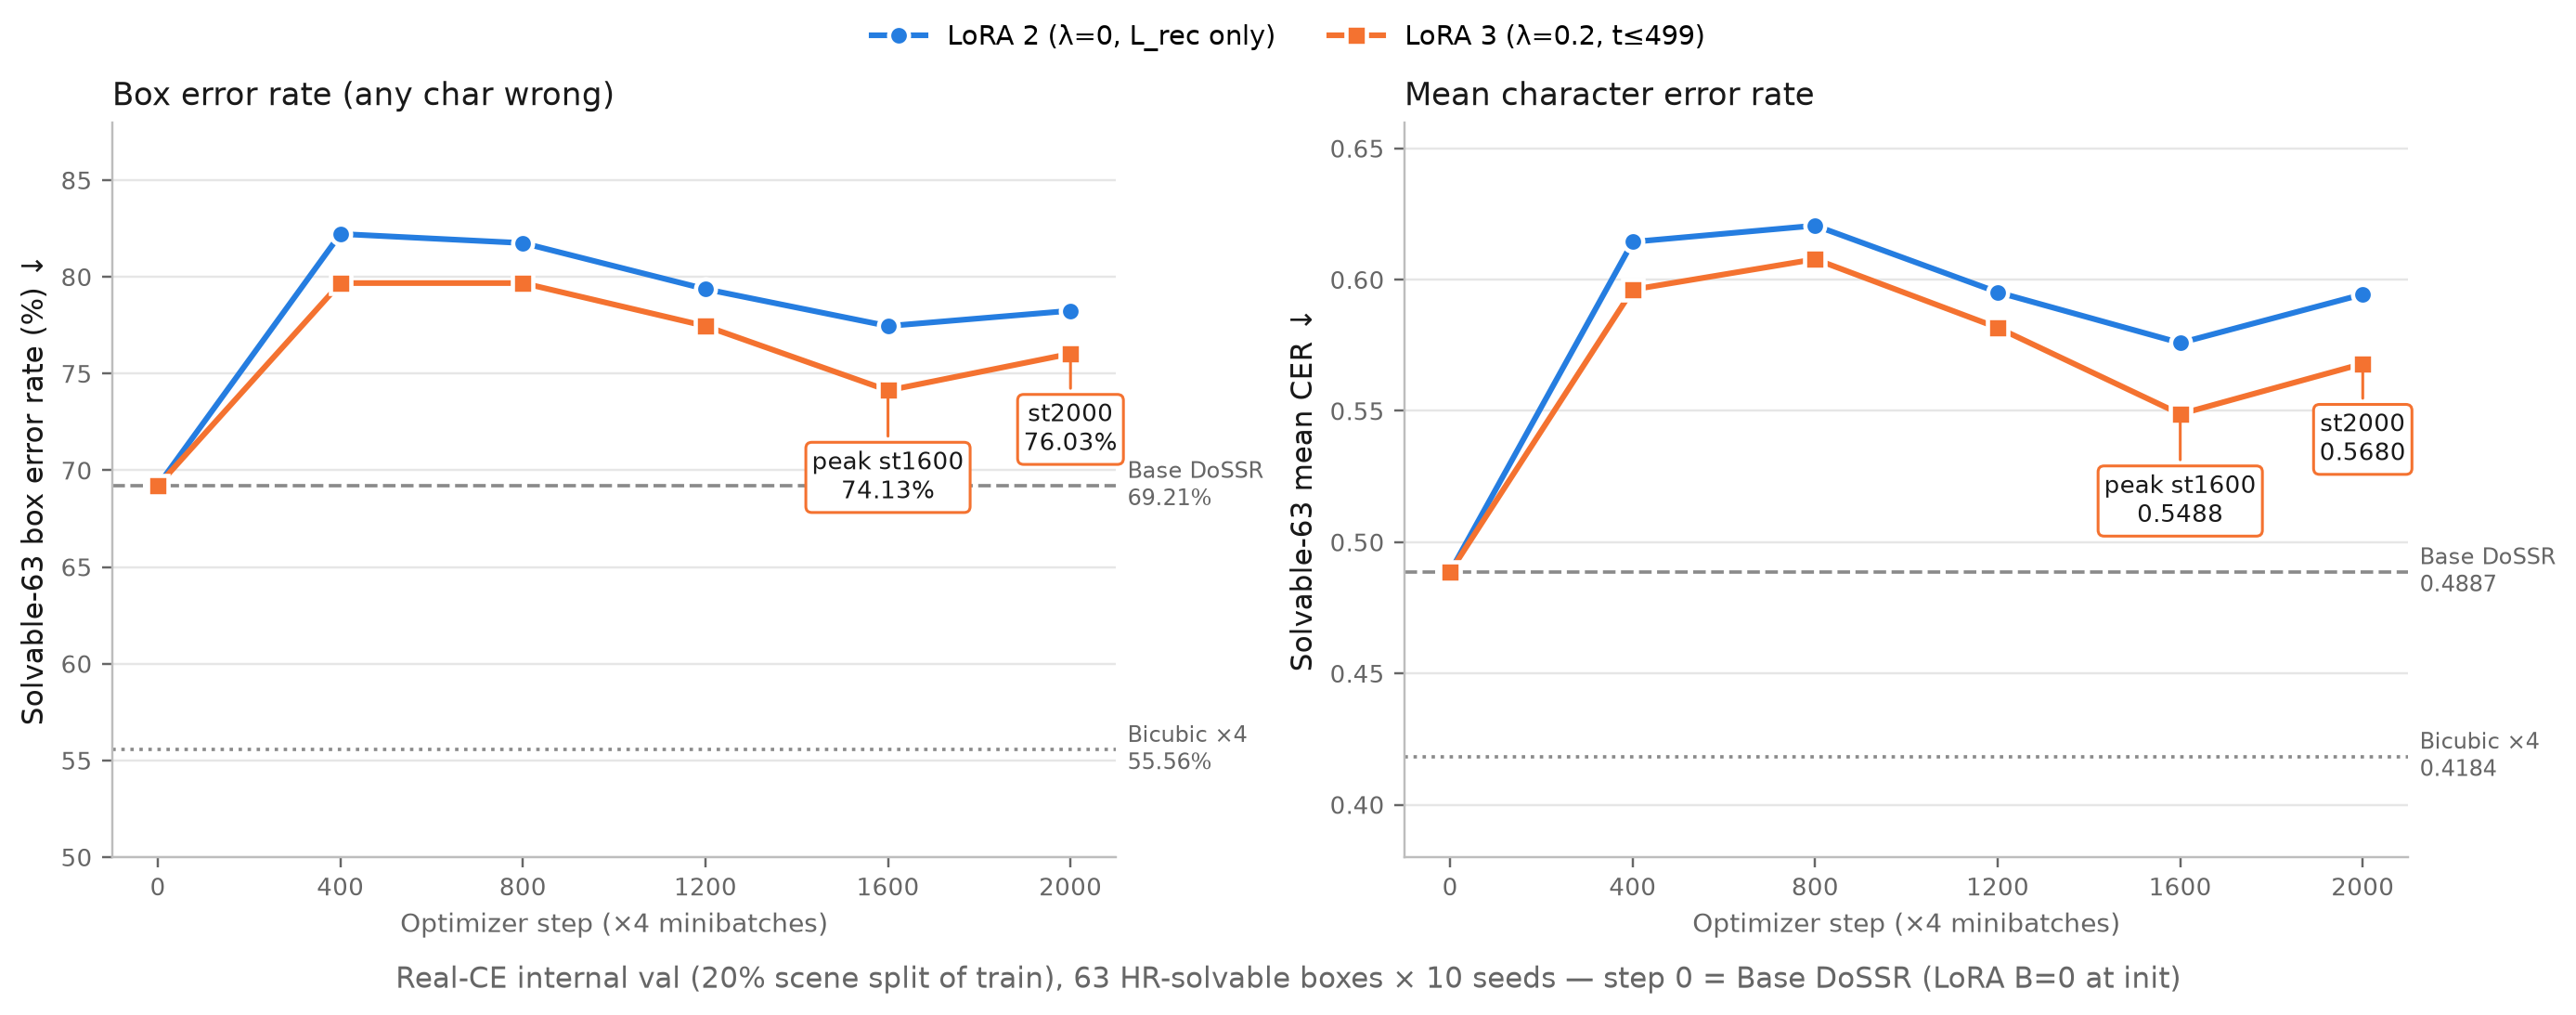
\includegraphics[width=0.95\linewidth]{figures/phase2_curve1_ocr_boxerr_cer.png}\\[6pt]
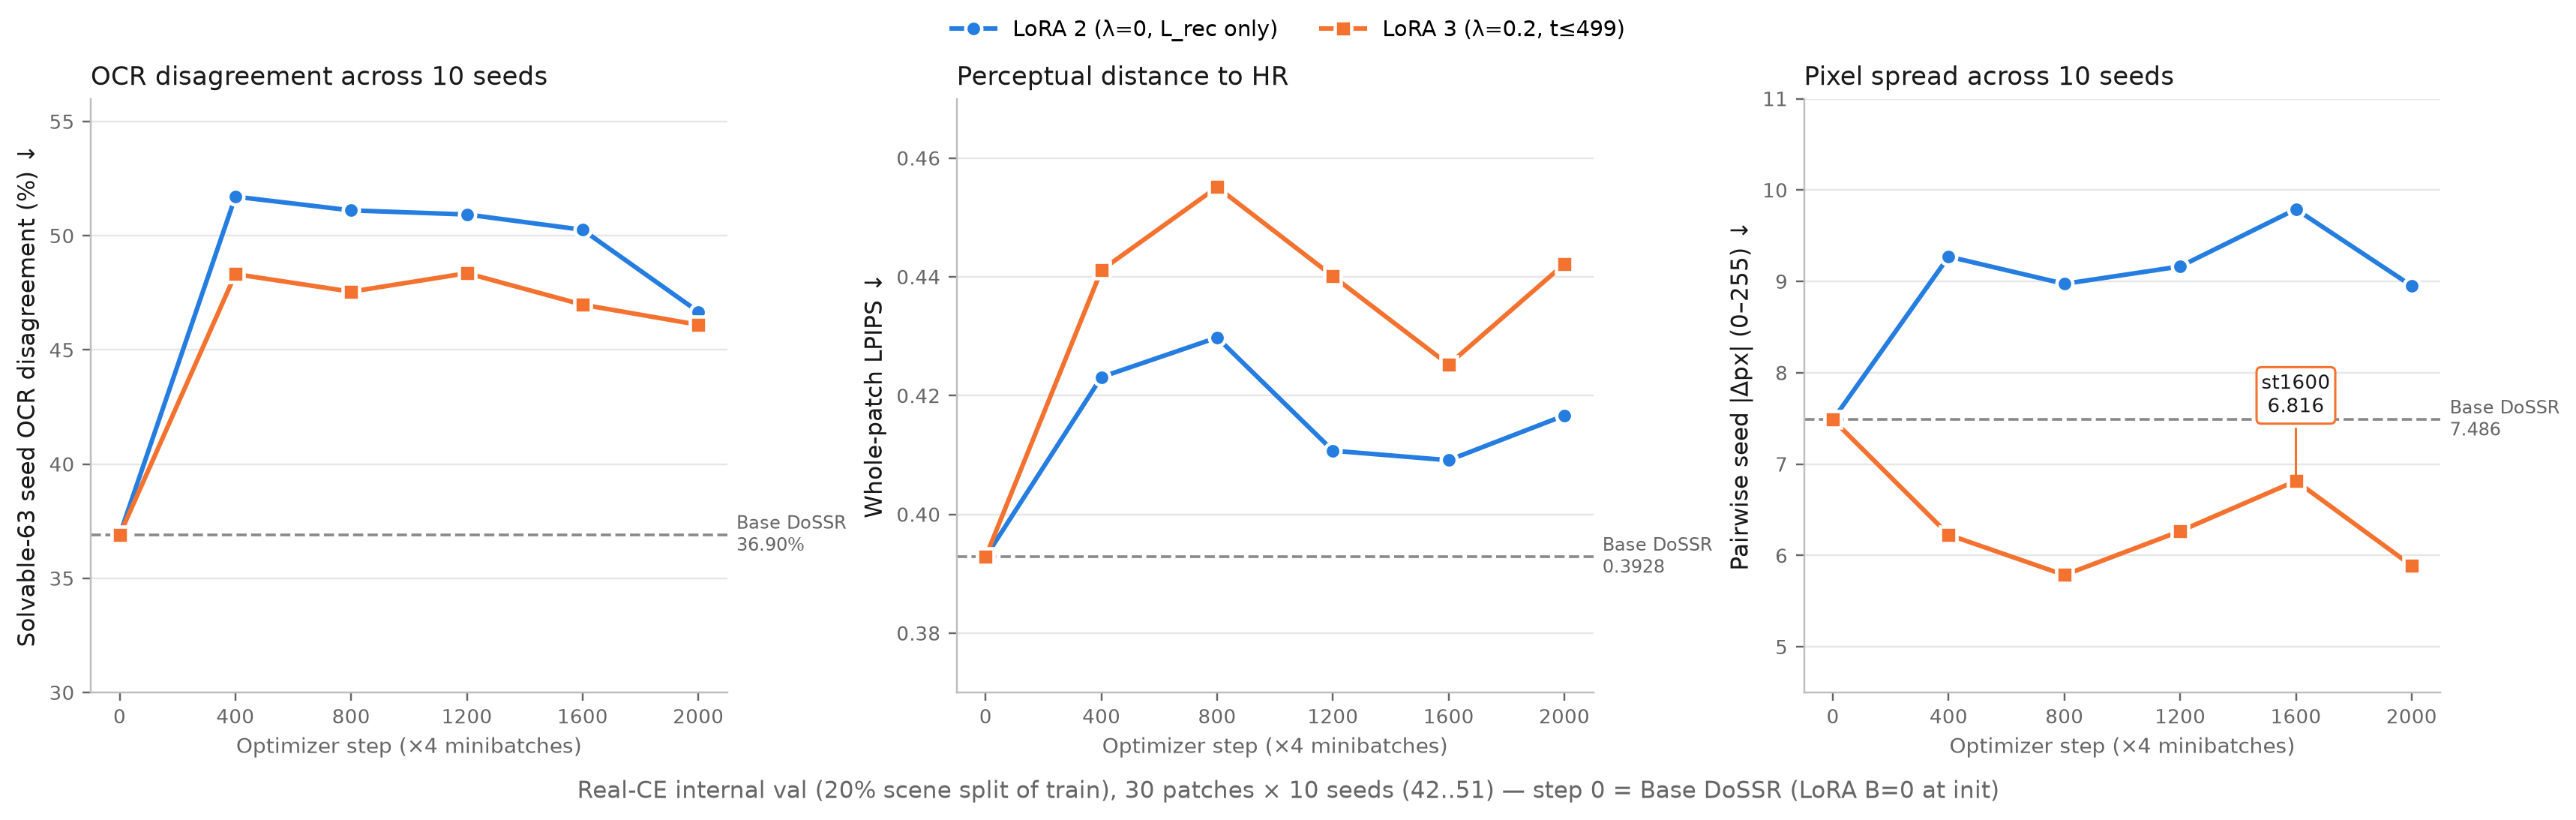
\includegraphics[width=0.95\linewidth]{figures/phase2_curve2_disag_lpips_pairpx.png}
\caption{Validation trajectories across 0--2,000 steps (step~0 equals Base DoSSR since LoRA $B=0$ at initialization). Top: Solvable-63 Box Error Rate and Mean CER (10 seeds) with Base DoSSR (dashed) and Bicubic~$\times 4$ (dotted) references. Bottom: Solvable-63 seed OCR disagreement, whole-patch LPIPS, and mean pairwise pixel spread (\texttt{pair\_px}).}
\label{fig:val_curves}
\end{figure}

\subsection{Diagnostic Category Breakdown (Solvable-63 Cohort)}
To test whether lowering $\lambda_{\text{cons}}$ to $0.2$ and gating $t \le 499$ eliminated the thin-stroke/digit degradation seen in the $\lambda=0.5$ pilot, Table~\ref{tab:categories} summarizes the four non-exclusive diagnostic categories on the 63 HR-solvable boxes: \texttt{numeric\_or\_date} (24 solvable / 50 total), \texttt{latin\_only} (16 / 67), \texttt{border\_touching} ($\le 16$~px from patch edge, 27 / 73), and \texttt{cjk\_signage} (35 / 68).

\begin{table}[ht]
\centering
\small
\caption{Diagnostic category metrics on the 63 HR-solvable boxes (Box Error Rate / Mean CER). Bold marks the best Box Error Rate and Mean CER separately among the diffusion/LoRA rows; Bicubic $\times 4$ achieves the lowest OCR error overall in all four categories.}
\label{tab:categories}
\resizebox{\textwidth}{!}{
\begin{tabular}{lcccc}
\toprule
Method / Checkpoint & \texttt{numeric\_or\_date} (24) & \texttt{latin\_only} (16) & \texttt{border\_touching} (27) & \texttt{cjk\_signage} (35) \\
\midrule
Bicubic $\times 4$ & 70.8\% / 0.4863 & 37.5\% / 0.2147 & 59.3\% / 0.5049 & 60.0\% / 0.4721 \\
Base DoSSR (unmodified) & \textbf{72.1\%} / \textbf{0.5347} & \textbf{61.9\%} / \textbf{0.2914} & \textbf{79.3\%} / \textbf{0.5918} & \textbf{75.4\%} / \textbf{0.5817} \\
LoRA~2 ($\lambda=0.0$, st0400) & 81.2\% / 0.5854 & 73.8\% / 0.4517 & 92.2\% / 0.7044 & 90.3\% / 0.7322 \\
LoRA~3 ($\lambda=0.5$, st0400 pilot) & 76.2\% / 0.5865 & 65.0\% / 0.4183 & 85.6\% / 0.6642 & 84.3\% / 0.6755 \\
\texttt{lora2\_s231\_st1600} & 77.1\% / 0.5581 & 68.8\% / 0.3991 & 85.6\% / 0.6701 & 85.4\% / 0.6834 \\
\texttt{lora3\_s231\_st1600} ($\lambda=0.2, t\le 499$) & 75.4\% / 0.5440 & 66.2\% / 0.3899 & 82.2\% / 0.6405 & 80.6\% / 0.6387 \\
\bottomrule
\end{tabular}
}
\end{table}

Crucially, \texttt{lora3\_s231\_st1600} reverses the $\lambda=0.5$ pilot regression on \texttt{numeric\_or\_date}, lowering Mean CER from $0.5865$ to $0.5440$ (close to \texttt{Base DoSSR} at $0.5347$) and beating \texttt{lora2\_s231\_st1600} on both Box Error Rate and Mean CER across all four categories, while \texttt{Base DoSSR} still leads all LoRA runs in every category. Relative to pilot \texttt{LoRA~2} (\texttt{st0400}), \texttt{lora3\_s231\_st1600} incurs zero Solv-63 Box Error regressions in every category (\texttt{6/18/0} on \texttt{numeric\_or\_date}, \texttt{8/8/0} on \texttt{latin\_only}, \texttt{10/17/0} on \texttt{border\_touching}, and \texttt{10/25/0} on \texttt{cjk\_signage}; full \texttt{All-154} and \texttt{Solvable-63} tables are archived in \path{docs/m2_phase2_category_and_wtl_tables.md}).

\subsection{Qualitative Visual Crop Inspection}
Tracked validation highlight boxes (\path{phase2_2000step_curves_s231.json}) illustrate both regimes: on thin slashes in \path{ip12pro_output_100APPLE_renew_29_patch000.png} (box~1, \texttt{"2024/06/17"}), \texttt{LoRA~3} improves over \texttt{LoRA~2} at step~400 ($0.5400$ vs.\ $0.5700$ CER) before extended training over-smooths fine slashes by step~2,000 ($0.9200$ CER); conversely, on thicker signage strokes in \path{ip11pro_output_TextSR_renew_114_patch000.png}, box~1 (\texttt{"paas"}) reaches $50.0\%$ Box Error at \texttt{LoRA~3} steps~1,200/2,000 (improving over \texttt{Base DoSSR}'s $60.0\%$) and box~5 (8-character CJK sentence) lowers CER to $0.7500$ at \texttt{st1600} (beating \texttt{Base DoSSR}'s $0.7750$).

\section{Compute, VRAM, and Timing Audit}
Table~\ref{tab:compute} reports NVIDIA L4 resource usage (\texttt{22.5~GiB} VRAM, \texttt{seed=231}, \texttt{grad\_accum=4}), showing $+0.00$~GiB extra peak VRAM ($8.04$ / $8.52$~GiB) from our two-pass backward. Adding $\mathcal{L}_{\text{cons}}$ raised step time by $+15.20\%$ in the $\lambda=0.5$ full-$t$ pilot ($4.67$ vs.\ $5.38$~s/step, \path{results/lora_pilot_summary.json}) and by $+7.65\%$ in the 2,000-step gated run ($4.7407$ vs.\ $5.1035$~s/step). Because those runs were in different Colab sessions with different base speeds, that comparison is only rough, though within Phase~2 gating $t \le 499$ lowered \texttt{LoRA~3} from $5.4357$ to $5.1045$~s/step. Because the paired 2,000-step study plus ten 10-seed evaluations used $\sim 7$~hours of L4 quota, the second training seed (\texttt{seed=777}) was not run.

\begin{table}[ht]
\centering
\small
\caption{Phase-2 NVIDIA L4 hardware, timestep gating, and wall-time audit (\texttt{seed=231}, \texttt{grad\_accum=4}).}
\label{tab:compute}
\resizebox{\textwidth}{!}{
\begin{tabular}{lccccccc}
\toprule
Run Identifier & Steps / Minibatches & Mean sampled $t$ & Share with $t<500$ & Active $\mathcal{L}_{\text{cons}}$ & Peak VRAM (Alloc / Res) & Mean / p95 \texttt{s/step} & Est.\ Wall Time \\
\midrule
\texttt{lora3-t499-pilot} & 400 / 1,600 & 488.89 & $814/1{,}600$ ($50.88\%$) & \textbf{50.88\%} & 8.04 / 8.52 GiB & \textbf{5.1045 / 5.4376 s} & 34.0 min \\
\texttt{lora2-full2000-s231} & 2,000 / 8,000 & 502.16 & $3{,}948/8{,}000$ ($49.35\%$) & 0.00\% & 8.04 / 8.52 GiB & 4.7407 / 4.7931 s & 2.63 hr \\
\texttt{lora3-full2000-s231} & 2,000 / 8,000 & 502.16 & $3{,}948/8{,}000$ ($49.35\%$) & \textbf{49.35\%} & \textbf{8.04 / 8.52 GiB ($+0.00$)} & \textbf{5.1035 / 5.4305 s} & 2.84 hr \\
\bottomrule
\end{tabular}
}
\end{table}

\section{Honest Comparison, Limitations, Diagnosis, and Next Steps}
\paragraph{What Worked, What Did Not, and Comparison with Bicubic $\times 4$:} Within LoRA fine-tuning, $\mathcal{L}_{\text{cons}}$ beats \texttt{LoRA~2} at every checkpoint (400--2,000) with $+0.00$~GiB extra VRAM, reaches its best OCR at step~1,600 in our run ($-3.33$~pp Solv-63 BoxErr vs.\ \texttt{LoRA~2}; $20/43/0$ W/T/L), and avoids the $\lambda=0.5$ pilot blur. Compared to \texttt{Base DoSSR}, \texttt{lora3\_s231\_st1600} reaches higher $\text{PSNR}_Y$ ($17.7842$ vs.\ $17.6307$~dB) and $\text{SSIM}_Y$ ($0.6652$ vs.\ $0.6345$), and lowers cross-seed spread ($\text{pair\_px} = 6.816$ vs.\ $7.486$; $\text{pair\_lpips} = 0.1183$ vs.\ $0.1267$), though lower \texttt{pair\_px} can come from blurrier images and is not a clear win by itself. However, \texttt{lora3\_s231\_st1600} has worse LPIPS than \texttt{Base DoSSR} ($0.4252$ vs.\ $0.3928$), and \texttt{Base DoSSR} still beats all LoRA runs on OCR ($69.21\%$ vs.\ $74.13\%$ Solv-63 BoxErr; $36.90\%$ vs.\ $46.98\%$ Disagreement). Finally, \texttt{Bicubic} $\times 4$ ($55.56\%$ Solv-63 BoxErr, $0.4184$ CER) beats both \texttt{Base DoSSR} and all LoRA runs on OCR, because bicubic only blurs existing strokes while diffusion can invent sharp-looking strokes that turn into wrong characters.

\paragraph{Likely Cause (Untested) and Study Limits:} Phase~2 gated $\mathcal{L}_{\text{cons}}$ to $t \le 499$, but $\mathcal{L}_{\text{rec}}$ stayed active across uniform $t \in [0, 999]$. As a result, $50.65\%$ ($4{,}052 / 8{,}000$) of minibatches updated LoRA on dead timesteps $t \ge 500$, where $1 - \eta_t \equiv 0$, $x_{\text{rect}}(t) = \hat{x}_{\text{LR}}$ carries zero HR signal, and the 5-step \texttt{SpacedSampler} ($t \in \{499, 399, 299, 200, 100\}$) never runs. This drift may explain the early $-13.01$~pp OCR gap in \texttt{LoRA~2 st0400} ($82.22\%$ vs.\ \texttt{Base DoSSR} $69.21\%$) that $\mathcal{L}_{\text{cons}}$ only partly closed ($82.22\% \to 74.13\%$). Note that upstream DoSSR pretraining samples the same $t \in [0, 999]$ range with the same L1 loss (\path{external/DOSSR/model/cldm.py:346--353}), so dead-timestep drift is a working hypothesis alongside alternative causes such as $\alpha_{\text{text}}=5$, FP16 training, and the small training split. Next Step~1 below is the direct test of this hypothesis. Finally, training used a single seed (\texttt{231}; \texttt{seed=777} was not run) and validation covers only 63 HR-solvable boxes, so small 1--3~pp differences may be noise.

\paragraph{Immediate Next Steps:} (1)~If approved by the mentor, test gating \emph{both} $\mathcal{L}_{\text{rec}}$ and $\mathcal{L}_{\text{cons}}$ to $t \le 499$ with a lower learning rate or cosine decay; (2)~run final evaluation once on the untouched $300$-pair official \texttt{RealCE/val} set and \texttt{RealSRVal\_crop128}.

\section{Reproducibility Guide}
All Phase-2 checks, training runs, and evaluation summaries are reproducible via:
\begin{verbatim}
# 1. Exact eta_t / SpacedSampler audit & CPU FP32 gradient equivalence
python src/lora_text_loss.py --audit-eta-schedule
python src/lora_text_loss.py --run-cpu-tests --verify-fp32-gradients

# 2. Scene-disjoint split (645 train -> 80/20, seed=42; 300 val untouched)
python scripts/split_realce_by_scene.py --split train --scale x4 \
  --val-ratio 0.20 --seed 42

# 3. 2,000-step LoRA 3 run (lambda=0.2, t<=499, grad_accum=4)
python scripts/run_lora_trial.py --config configs/lora3_full2000_s231.yaml \
  --verify-fp32-grad --cons-t-max 499

# 4. Standardized OCR evaluation & Phase-2 curve aggregation
python scripts/text_eval.py --ocr-backend rapidocr --rec-only \
  --rotate-vertical --upscale 2
python scripts/analyze_realce_lora_sweep.py
\end{verbatim}

\enlargethispage{2\baselineskip}
\begingroup
\footnotesize
\setlength{\itemsep}{0pt}
\begin{thebibliography}{9}
\bibitem{sun2024ccsr}
Sun et al., ``Improving the Stability and Efficiency of Diffusion Models for Content Consistent Super-Resolution,'' arXiv:2401.00877, 2024.\
\url{https://arxiv.org/abs/2401.00877}

\bibitem{jiang2025pnfs}
Jiang et al., ``Restabilizing Diffusion Models with Predictive Noise Fusion Strategy for Image Super-Resolution,'' in \emph{Proceedings of the AAAI Conference on Artificial Intelligence}, vol.~39, no.~4, pp.~4021--4029, 2025.\
\url{https://doi.org/10.1609/aaai.v39i4.32421}

\bibitem{hu2025tadIsr}
Hu et al., ``Text-Aware Real-World Image Super-Resolution via Diffusion Model with Joint Segmentation Decoders,'' in \emph{Advances in Neural Information Processing Systems}, 2025.\
\href{https://proceedings.neurips.cc/paper_files/paper/2025/hash/58ce6a4b9c16d11975f11e4a23871041-Abstract-Conference.html}{NeurIPS proceedings page}
\end{thebibliography}
\endgroup

\end{document}
